\documentclass[cn,cyan,fleqn]{elegantbook}
\usepackage{amsmath}
\usepackage{ntheorem}
\usepackage{array}
\usepackage{booktabs}
\usepackage{times}
\usepackage{fontspec}
\usepackage{libertine}
\usepackage{pgf} % for the calculation
\usepackage{extarrows}
\usepackage{tikz}
\usepackage{extarrows}
\usepackage{array}%需要该宏包
\usepackage{xr}
\usepackage{ctex}
\usepackage{CJK}
\usepackage{mathpazo}
\usepackage{tikz}
\newcommand*{\circled}[1]{\lower.7ex\hbox{\tikz\draw (0pt, 0pt)%
    circle (.5em) node {\makebox[1em][c]{\small #1}};}}
\newcommand*{\num}{pi}
 % define the plot style and the axis style
\tikzset{elegant/.style={smooth,thick,samples=50,blue}}
\tikzset{eaxis/.style={->,>=stealth}}
\DeclareMathSizes{12}{21}{15}{11}
\title{考研高等数学笔记}
\subtitle{GRE Advanced Mathematics Note}

\author{BasinChen}
\institute{中国高校联盟}
\date{\today}
\version{3.07}

\equote{Victory won\rq t come to us unless we go to it. --- M. Moore}

\logo{logo.png}
\cover{cover.jpg}

\usepackage[authoryear]{gbt7714}

\begin{document}
\maketitle
\tableofcontents

% \thispagestyle{empty}

\mainmatter
\hypersetup{pageanchor=true}
\chapter{极限}
\section{函数极限的定义}
\begin{definition}{极限}{}
\[\lim\limits_{x \to \cdot}f(x)=A\hspace{1cm}\mbox{其中} \left\{ \begin{array}{l}
                                             x\to x_0 \\
                                             x\to \infty
                                           \end{array}\right. \hspace{1cm}\mbox{满足} \forall \varepsilon > 0\; , \;x \to \cdot \;,\; |f(x)-A|<\varepsilon\]
\end{definition}
\textbf{性质}:\par
\textsl{\textcolor{third}{1. $A$的唯一性:极限若存在,必唯一。}}\\
\[
\mbox{应用}\left\{ \begin{array}{l}
    \mbox{左右极限} \\
    \mbox{导数}
  \end{array}\right. \]
  \textbf{例如}:
  \[
  \lim\limits_{x\to 0}\frac{\tan \pi x}{|x|(x^2-1)}\hspace{1cm} I_+=\lim\limits_{x\to0^+}\frac{\pi x}{x(x^2-1)}=-\pi\hspace{0.5cm}\mbox{同理可得}\hspace{0.5cm}I_-
=\pi  \]\par
\textsl{\textcolor{third}{2. $A$是一个数!}}\\
\[ \lim\limits_{x\to\cdot}f(x)=A \]
\begin{problem}
\begin{equation}\nonumber
\begin{aligned}
&\mbox{已知}\lim\limits_{a\to 1}f(x)\mbox{存在}, f(x)=\frac{x-\arctan(x-1)-1}{(x-1)^3}+2x^2e^{x-1}\cdot\lim\limits_{x\to 1}f(x) \\
&\mbox{求}\displaystyle f(x):
\end{aligned}
\end{equation}
\end{problem}
\begin{solution}
\begin{equation}\nonumber
\begin{aligned}
&\mbox{记:} \lim\limits_{x\to 1}f(x)=A, \mbox{所以}\lim\limits_{x\to 1}f(x)=\frac{(x-1)-\arctan(x-1)}{(x-1)^3}+2A \\
&\Rightarrow \lim\limits_{t\to 0}f(x)=\frac{t-\arctan t}{t^3}+2A=\frac{1}{3}+2A=A \\
&\Rightarrow A=-\frac{1}{3}
\end{aligned}
\end{equation}
\end{solution}
\textsl{\textcolor{third}{3. 有界性}}\\
\[ \lim\limits{x\to \cdot}\hspace{0.5cm}|f(x)|\leqslant M \]
\begin{problem}
\begin{equation}
\mbox{若}\lim\limits_{x\to x_0}=\frac{f(x)}{x-x_0}=A  \; \mbox{(存在)} ,\mbox{求}\; \lim\limits_{x\to x_0}f(x)\\
\end{equation}
\end{problem}
\begin{solution}
\begin{equation}
=\lim\limits_{x\to x_0}\frac{f(x)}{x-x_0}(x-x_0)=0 \; \mbox{(有界乘以无穷小)}
\end{equation}
\end{solution}
\par

\textsl{\textcolor{third}{4.保号性}}\\
通俗说来,$x \to \cdot $\;  时 ,若$A>0$,$f(x)>0$\;(局部)不等式脱帽法,即:
\[
\lim\limits_{x\to \cdot}f(x)=A>0\;\Rightarrow\; f(x)>0\;(x\to \cdot)
\]
\begin{problem}
\begin{equation*}
       \mbox{证明:当}x\to 0^+,0<\tan^2x-x^2<x^4 \; \mbox{成立}.\\
\end{equation*}
\end{problem}
\begin{solution}
\begin{equation*}
\begin{aligned}
       &\mbox{分析:} \lim\limits_{x\to 0^+}\frac{tan^2x-x^2}{x^4}=\lim\limits_{x\to 0^+}\frac{(\tan x+x)(\tan x-x)}{x\cdot x^3}=\frac{2}{3}<1\\
       &\mbox{故}\lim\limits_{x\to 0^+}\big[ \frac{\tan^2x-x^2}{x^4}-1 \big]<0\Rightarrow\frac{\tan^2x-x^2}{x^4}-1<0  \\
       &\mbox{即}\tan^2x-x^2<x^4\\
       &\mbox{又}x\to 0^+\; \tan x>x \\
       &\Rightarrow 0<\tan^2x-x^2<x^4
\end{aligned}
\end{equation*}
\end{solution}
\par
\textsl{\textcolor{third}{5.等式脱帽}}\\
$\Leftrightarrow\hspace{1cm}\displaystyle f(x)=A+\alpha \hspace{1cm}\lim\limits_{x\to \cdot}\alpha=0$\\
\textbf{注} 1.主要适用于抽象函数$f(x)$,多用于已知某一极限求另一极限。2.$f(x, y)$\\
\begin{problem}
\begin{equation}
\mbox{设} \lim\limits_{x\to 0}\frac{\ln [1+\frac{f(x)}{\sin x}]}{a^x-1}=A\hspace{1cm} a>0\hspace{0.5cm} a\neq1 , \mbox{求} \lim\limits_{x\to 0}\frac{f(x)}{x^2} \\
\end{equation}
\end{problem}
\begin{solution}
\begin{equation*}
\begin{aligned}
  &\displaystyle \mbox{分析: 等式脱帽法,解出}f(x)\;\\
   &\mbox{即 } \frac{\ln[1+\frac{f(x)}{\sin x}]}{a^x-1}=A+\alpha \;\\
    &\mbox{其中}\;\lim\limits_{x\to 0}\alpha=0\; \ln[1+\frac{f(x)}{\sin x}]=(a^x-1)(A+\alpha) \\
       &\Rightarrow 1+\frac{f(x)}{\sin x}=e^{(a^x-1)(A+\alpha)}\; , f(x)=[e^{(a^x-1)(A+\alpha)}-1]\sin x \\
       &\mbox{则}\; \lim\limits_{x\to 0}\frac{f(x)}{x^2}=\lim\limits_{x\to 0}\frac{((e^{(a^x-1)(A+\alpha)}-1))\sin x}{x^2}=x\ln a \\
       & =\lim\limits_{x\to 0}\frac{(a^x-1)(A+\alpha)}{x}=A\ln a
\end{aligned}
\end{equation*}
\end{solution}
\section{函数极限的计算}
七种未定式:\[ \frac{0}{0},\; \frac{\infty}{\infty},\; \infty\cdot0,\; \infty-\infty,\; \infty^0,\; 0^0,\; 1^\infty \]
\uppercase\expandafter{\romannumeral1}.先化简:\par
(1)\;等价替换 (当$x\to 0$时)
\begin{equation}\nonumber
  \begin{aligned}
  \sin x    &\sim x \hspace{1cm} &1-\cos x            &\sim \frac{1}{2}x^2\\
  \arcsin x &\sim x \hspace{1cm} &\arctan x           &\sim x\\
  \ln(1+x)  &\sim x \hspace{1cm} &e^x-1               &\sim x\\
  a^x-1     &\sim x\ln a \hspace{1cm} &(1+x)^\alpha-1 &\sim \alpha x\\
  \bigstar\mbox{若} \alpha&=o(\beta) \mbox{即} \lim\limits_{x\to \cdot }\frac{\alpha}{\beta}\overset{"\frac{0}{0}"}{=}0
  \end{aligned}
\end{equation}
\par
(2)\;化简
\[
\left\{
\begin{matrix}
        \mbox{提取公因式}\\
       \mbox{换元}\\
        \mbox{通分}\\
        u^v=e^{v\ln u}\\
        \mbox{公式}\\
\end{matrix}
\right.\hspace{1cm}
\mbox{换元}\left\{ \begin{matrix}
                   x=\frac{1}{t}\\
                    x-x_0=t\\
                    a^n-b^n\mbox{因式分解}\\%=(a-b)(a^{n-1}+a^{n-2}b+\dots+ab^{n-2}+b^{n-1})\\%(a-b)\\
                    \mbox{有理化}\sqrt{a}-\sqrt{b}=\frac{a-b}{\sqrt{a}+\sqrt{b}}
                 \end{matrix} \right.
                 \]\par
(3)\;及时提出极限不为0的因式\\
\uppercase\expandafter{\romannumeral2}.洛必达法则:
%%%%%%%%%%%%%%%%%%%%%%%%%%%%%%%%%%%%%%%%%%%%%%
\begin{equation*}
\begin{aligned}
1.\;& \lim\limits_{x\to \cdot}\frac{f(x)}{g(x)}\overset{"\frac{0}{0}"}{=}\lim\limits_{x\to\cdot}\frac{f'(x)}{g'(x)}\\
2.\;& \lim\limits_{x\to a}\frac{\int_{a}^{x}f(t)\text{d}t}{\int_{a}^{x}g(t)\text{d}t}\overset{"\frac{0}{0}"}{=}\lim\limits_{x\to a}\frac{f(x)}{g(x)}\\
3.\;& \lim\limits_{x\to a}\frac{\int_{a}^{\phi(x)}f(t)\text{d}t}{\int_{a}^{\psi(x)}g(t)\text{d}t}=\lim\limits_{x\to a}\frac{f(\phi(x))\phi'(x)}{g(\psi(x))\psi'(x)}\\
\end{aligned}
\end{equation*}
\begin{problem}
\begin{equation}
\lim\limits_{x \to 0}\frac{(3+2\tan x)^2-3^x}{3sin^2x+x^3\cos\frac{1}{x}}\hspace{0.5cm}(\frac{0}{0}\mbox{型}) \\
\end{equation}
\end{problem}
\begin{solution}
\begin{equation*}
\begin{aligned}
       & \mbox{[分析]}\mbox{由于}\lim\limits_{x\to 0}\frac{x^3cos\frac{1}{x}}{3\sin^2x}=\frac{1}{3}\lim\limits_{x\to 0}x\cos\frac{1}{x}=0\\
       & \xLongrightarrow{\frac{\mbox{高阶}}{\mbox{低阶}}} x^3\cos\frac{1}{x}=o(3\sin^2x)\\
       & \therefore 3\sin^2x+x^3\cos\frac{1}{x} \sim 3\sin^2x \sim 3x^2\\
       & \mbox{原式}=\lim\limits_{x\to 0}\frac{3^x[(1+\frac{2}{3}\tan x)^x-1]}{3x^2}=\lim\limits_{x\to 0}\frac{e^{x\ln(1+\frac{2}{3}\tan x)}-1}{3x^2}\\
       &=\lim\limits_{x\to 0}\frac{x\ln(1+\frac{2}{3}\tan x)}{3x^2}\\
       & =\lim\limits_{x\to 0}\frac{x\cdot\frac{2}{3}\tan x}{3x^2}=\frac{2}{9}
\end{aligned}
\end{equation*}
\end{solution}
\begin{problem}
\begin{equation*}
\lim\limits_{x\to 0}\int_{0}^{x}\frac{\sin 2t}{\sqrt{4+t^2}\int_{0}^{x}(\sqrt{t+1}-1)\text{d}t}\text{d}t \\
\end{equation*}
\end{problem}
\begin{solution}
\begin{equation*}
\begin{aligned}
 & \Rightarrow \lim\limits_{x\to 0}\frac{\int_{0}^{x}\frac{\sin 2t}{\sqrt{4+t^2}}\text{d}t}{\int_{0}^{x}(\sqrt{t+1}-1)\text{d}t}=\mbox{(洛)}\lim\limits_{x\to 0}\frac{\frac{\sin 2x}{\sqrt{4+x^2}}}{\sqrt{x+1}-1}=\lim\limits_{x\to 0}\frac{\sin 2x}{\sqrt{4+x^2}(\sqrt{x+1}-1)}=2
\end{aligned}
\end{equation*}
\end{solution}
\begin{problem}
\begin{equation*}
\lim\limits_{x\to 3^+}\frac{\cos x\cdot \ln(x-3)}{\ln(e^x-e^3)}\;\;(\frac{\infty}{\infty}) \\
\end{equation*}
\end{problem}
\begin{solution}
\begin{equation*}
\begin{aligned}
 & =\cos 3\cdot\lim\limits_{x\to 3^+}\frac{\ln(x-3)}{\ln(e^x-e^3)}=\cos 3\cdot\lim\limits_{x\to 3^+}\frac{1}{x-3}\cdot\frac{e^x-e^3}{e^x}=\frac{1}{e^3}\cos 3\cdot\lim\limits_{x\to 3^+}\frac{e^x-e^3}{x-3}\\
       & =\frac{\cos 3}{e^3}\lim\limits_{x\to 3^+}\frac{e^x}{1}=\cos 3\\
       & \mbox{[及时提出极限不为0的因式]}
\end{aligned}
\end{equation*}
\end{solution}
\begin{problem}
\begin{equation*}
\lim\limits_{x\to 0}(\frac{1+x}{1-e^x}-\frac{1}{x})\;\;(\infty-\infty) \\
\end{equation*}
\end{problem}
\begin{solution}
\begin{equation*}
\begin{aligned}
       & \mbox{[分析] \; 有分母,则通分}\\
       & \mbox{原式}=\lim\limits_{x\to 0}\frac{x+x^2-1+e^{-x}}{(1-e^{-x})\cdot x}=\lim\limits_{x\to 0}\frac{1+2x-e^{-x}}{2x}=1+\frac{1}{2}=\frac{3}{2}
\end{aligned}
\end{equation*}
\end{solution}
\begin{problem}
\begin{equation*}
\lim\limits_{x\to\infty}e^{-x}(1+\frac{1}{x})^{x^2}\hspace{0.5cm}u^v=v\ln n \\
\end{equation*}
\end{problem}
\begin{solution}
\begin{equation*}
\begin{aligned}
       & \mbox{原式}=\lim\limits_{x\to 0}e^{-x}\cdot e^{x^2\ln(1+\frac{1}{x})}\\
       & =e^{\lim\limits_{x\to \infty}[x^2\ln(1+\frac{1}{x})-x]}\overset{x=\frac{1}{t}}{=}e^{\lim\limits_{t\to 0}[\frac{\ln(1+t)}{t^2}-\frac{1}{t}]}\\
       & e^{\lim\limits_{t\to 0}[\frac{\ln(1+t)-t}{t^2}]}=e^{-\frac{1}{2}}
\end{aligned}
\end{equation*}
\end{solution}
\begin{problem}
\begin{equation*}
\lim\limits_{x\to 0^+}x^{\ln(\frac{\ln x-1}{\ln x+1})}\hspace{0.5cm}(0^0)
\end{equation*}
\end{problem}
\begin{solution}
\begin{equation*}
\begin{aligned}
&u^v=r^{v\ln u}\\
&e^{\lim\limits_{x\to 0}\ln(\frac{\ln x-1}{\ln x+1})\cdot\ln x}\\
&=e^{\lim\limits_{x\to 0}\ln(1-\frac{2}{\ln x+1})\cdot\ln x}\\
&=e^{\lim\limits_{x\to 0}\frac{-2\ln x}{1\cdot\ln x+1}}=e^{-2}\\
\end{aligned}
\end{equation*}
\end{solution}
\begin{problem}
\begin{equation*}
\lim\limits_{x\to 0^+}(\frac{\sin x}{x})^{\frac{1}{1-\cos x}}\hspace{0.5cm}(1^\infty)
\end{equation*}
\end{problem}
\begin{solution}
\begin{equation*}
\begin{aligned}
&\lim u^v\overset{1^\infty}{=}e^{\lim v\ln u}=e^{\lim v(\ln(1+u-1))}\\
&=e^{\lim v(u-1)}\\
&\mbox{原式}=e^{\lim\limits_{x\to 0^+}\frac{1}{1-\cos x}(\frac{\sin x}{x}-1)}\\
&=e^{\lim\limits_{x\to 0^+}\frac{\sin x-x}{\frac{1}{2}x^2\cdot x}}=e^{-\frac{1}{3}}
\end{aligned}
\end{equation*}
\end{solution}
\uppercase\expandafter{\romannumeral3}.泰勒公式:
\[f(x)=(\hspace{0.6cm})x^0+(\hspace{0.6cm})x^1+\dots+(\hspace{0.6cm})x^n+\dots\hspace{1cm}\mbox{其中,}x^\alpha\mbox{成为“基”}\]
(1)熟记公式
\begin{equation}\nonumber
  \begin{aligned}
  e^x&=1+x+\frac{x^2}{2!}+\frac{x^3}{3!}+\dots+\frac{x^n}{n!}+\dots=\sum_{n=0}^{\infty}\frac{x^n}{n!}\\
  \sin x&=x-\frac{1}{3!}x^3+\frac{1}{5!}x^5+\dots+(-1)^n\frac{x^{2n+1}}{(2n+1)!}=\sum(-1)^n\frac{x^{2n+1}}{(2n+1)!}\\
  \cos x&=1-\frac{1}{2!}x^2+\frac{1}{4!}x^4-\dots+(-1)^n\frac{x^{2n}}{2n!}\\
  \ln(1+x)&=x-\frac{1}{2}x^2+\frac{1}{3}x^3-\dots+(-1)^n\frac{x^n}{n}\\
  (1+x)^\alpha &=1+\alpha x+\frac{\alpha(\alpha-1)}{2}x^2+o(x^2)\\
  \tan x&=x+\frac{1}{3}x^3+o(x^3)\\
  \arctan x&=x-\frac{1}{3}x^3+o(x^3)\\
  \frac{1}{1-x}&=1+x+x^2+\dots+x^n\\
  \frac{1}{1+x}&=1-x+x^2-x^3+\dots+(-1)^nx^n+\dots\\
  \end{aligned}
\end{equation}
(2)展开原则\\
\textcolor{third}{$\displaystyle\frac{A}{B}$\;上下同阶原则}\\
\begin{problem}
\begin{equation*}
  \lim\limits_{x\to 0}\frac{1+\frac{1}{2}x^2-\sqrt{1+x^2}}{(\cos x-e^{\frac{x^2}{2}})\sin \frac{x^2}{2}}
\end{equation*}
\end{problem}
\begin{solution}
\begin{equation*}
  \mbox{原式}=\frac{-\frac{1}{8}x^4}{-\frac{x^4}{2}}
\end{equation*}
\end{solution}
\textcolor{third}{$\displaystyle A-B$型——幂次最低}\\
\begin{problem}
\begin{equation*}
  \cos x-e^{\frac{x^2}{2}}\sim ax^b\hspace{0.5cm}x\to 0
\end{equation*}
\end{problem}
\begin{solution}
\begin{equation*}
\begin{aligned}
  &\cos x=1-\frac{1}{2}x^2+o(x^2)\\
 & e^{\frac{x^2}{2}}=1+\frac{1}{2}x^2+o(x^2)\\
  &\cos x-e^{\frac{x^2}{2}}=-x^2+o(x^2)\\
\end{aligned}
\end{equation*}
\end{solution}
\begin{problem}
\begin{equation*}
  \lim\limits_{x\to \infty}(\sqrt[6]{x^6+x^5}-\frac{6}{x^6-x^5})
\end{equation*}
\end{problem}
\begin{solution}
\begin{equation*}
\begin{aligned}
 & \mbox{令}x=\frac{1}{t}:\\
 & \lim\limits_{t\to 0^+}(\sqrt[6]{\frac{1}{t^6}+\frac{1}{t^5}}-\sqrt[6]{\frac{1}{t^6}-\frac{1}{t^5}})\\
 & =\lim\limits_{t\to 0^+}\frac{\sqrt[6]{1+t}}{t}-\frac{\sqrt[6]{1-t}}{t}\\
  &=\lim\limits_{t\to 0^+}\frac{(1+t)^\frac{1}{6}-(1-t)^\frac{1}{6}}{t}\\
 & =\lim\limits_{t\to 0^+}\frac{1+\frac{1}{6}t-(1-\frac{1}{6}t)+o(t)}{t}\\
  &=\frac{1}{3}
\end{aligned}
\end{equation*}
\end{solution}
\textcolor{third}{无穷小比阶及其反问题}\\
\[\lim\limits_{x\to\cdot}\frac{f(x)}{g(x)}=(\frac{0}{0})\;\left\{ \begin{array}{l}0 \hspace{1cm}\mbox{高阶}\\
                                                                                c\neq 0\hspace{1cm}\mbox{同阶}\\
                                                                            \infty\hspace{1cm}\mbox{低阶}\end{array}\right.\]
\begin{problem}
\begin{equation}\nonumber
  \mbox{当}x\to 0^+\mbox{时}, \; \alpha=\int_{0}^{x}\cos t^2\text{d}t \; \beta=\int_{0}^{x^2}\tan \sqrt{t}\text{d}t \; \gamma=\int_{0}^{\sqrt{x}}\tan t^3\text{d}t
\end{equation}
\end{problem}
\begin{solution}
\begin{equation*}
  \begin{aligned}
  &\lim\limits_{x\to 0^+}\frac{\gamma}{\alpha}=\lim\limits_{x\to 0^+}\frac{\int_{0}^{\sqrt{x}}\sin^3 t\text{d}t}{\int_{0}^{x}\cos t^2\text{d}t}=\lim\limits_{x\to 0^+}\frac{\sin x^\frac{2}{3}\frac{1}{2\sqrt{x}}}{\cos x^2}=\lim\limits_{x\to 0^+}\frac{x^\frac{3}{2}}{x^\frac{1}{2}}=0\\
  &\Rightarrow\gamma\mbox{更高阶}\gamma=o(\alpha)\\
  &\lim\limits_{x\to 0^+}\frac{\beta}{\gamma}=\lim\limits_{x\to 0^+}\frac{\int_{0}^{x^2}\tan \sqrt{t}\mbox{d}t}{\int_{0}^{\sqrt{x}}\sin t^3\text{d}t}=\lim\limits_{x\to 0^+}\frac{\tan x\cdot 2x}{\sin x^\frac{3}{2}\cdot\frac{1}{2\sqrt{x}}}=0\\
  &\Rightarrow\beta=o(\gamma)\\
  &\beta>\gamma>\alpha
  \end{aligned}
\end{equation*}
\end{solution}
\section{函数极限的存在性}
\textcolor{third}{1.具体型,但洛必达法则失效——夹逼准则}
\begin{problem}
\begin{equation*}
  \begin{aligned}
  &\mbox{记:}s(x)=\int_{0}^{x}|\sin t|\text{d}t\\
  &(i)\mbox{证明:当}n\pi\leqslant x<(n+1)\pi\mbox{时}, 2n\leqslant s(x)\leqslant 2(n+1)\\
  &(ii)\mbox{求:}\lim\limits_{x\to \infty}\frac{\int_{0}^{x}|\sin t|\text{d}t}{x}
  \end{aligned}
\end{equation*}
\end{problem}
\begin{solution}
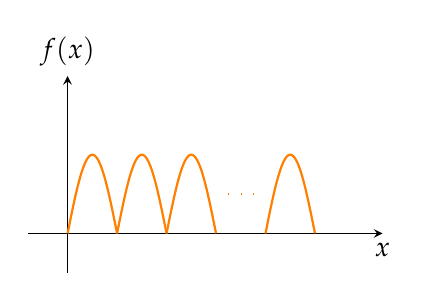
\begin{tikzpicture}
    \draw[eaxis] (-0.5,0) -- (4,0) node[below] {$x$};
    \draw[eaxis] (0,-0.5) -- (0,2) node[above] {$f(x)$};
    \draw[elegant,orange,domain=0:pi/5] plot(\x,{sin(5*\x r)});
    \draw[elegant,orange,domain=pi/5:2*pi/5] plot(\x,{sin(-5*\x r)});
    \draw[elegant,orange,domain=2*pi/5:3*pi/5] plot(\x,{sin(5*\x r)});
    \draw[elegant,orange,domain=2.042:2.0429] plot(\x,0.5);%,1.885,2.513
    \draw[elegant,orange,domain=2.199:2.1999] plot(\x,0.5);%,1.885,2.513
    \draw[elegant,orange,domain=2.356:2.3569] plot(\x,0.5);%,1.885,2.513
    \draw[elegant,orange,domain=4*pi/5:pi] plot(\x,{sin(5*\x r)});
\end{tikzpicture}
\begin{equation*}
 \begin{aligned}
  (i)&\mbox{由图可知:}S(n\pi)=n\cdot 2\\
  &[(n+1)\pi]=(n+1)\cdot 2\\
  &S'(x)>0\\
  &\mbox{当}n\pi\leqslant x\leqslant (n+1)\pi\\
  &2n=S(n\pi)\leqslant S(x)\leqslant S(n+1)\pi=2(n+1)\\
 (ii) &\mbox{由于:}2n\leqslant \int_{0}^{x}|\sin t|\text{d}t\leqslant 2(n+1) \; , \; \frac{1}{(n+1)\pi}\leqslant\frac{1}{x}\leqslant\frac{1}{n\pi}\\
  &\Rightarrow \frac{2n}{(n+1)\pi}\leqslant\frac{\int_{0}^{x}|\sin t|\text{d}t}{x}\leqslant\frac{2(n+1)}{n\pi}\\
  &n \to \infty \mbox{时,} \frac{2n}{(n+1)\pi}=\frac{2}{\pi}=\frac{2(n+1)}{n\pi}\\
  &\mbox{故:}\lim\limits_{x\to \infty}\frac{\int_{0}^{x}|\sin t|\text{d}t}{x}=\frac{2}{\pi}
  \end{aligned}
\end{equation*}
\end{solution}\newpage
\textcolor{third}{2.抽象型——单调有界准则}\\
\mbox{若}$\displaystyle f(x)$\mbox{递增,且有上界。则,}$\displaystyle \lim\limits_{x\to \infty}f(x)=\exists$
\begin{problem}
\begin{equation*}
  \begin{aligned}
  &\mbox{设,}x\geqslant 0, \; f(x) \mbox{满足}f'(x)=\frac{1}{x^+f^2(x)} \; f(0)=1 \;\mbox{证明}\\
  &(1).\;f'(x)\leqslant\frac{1}{1+x^2}\;\;\;x\geqslant 0\\
  &(2).\;\lim\limits_{x\to +\infty}f(x)\mbox{存在,且小于}1+\frac{\pi}{2}
  \end{aligned}
\end{equation*}
\end{problem}
\begin{solution}
\begin{equation*}
  \begin{aligned}
  &(1). \;\mbox{由于}f'(x)>0 \therefore f(x)\uparrow \therefore f'(x)=\frac{1}{x^2+f^2(x)} \leqslant \frac{1}{x^2+1}\\
  &(2). \;f(x)=f(a)+\int_{0}^{x}f'(t)\text{d}t\\
  &\therefore f(x)=f(0)+\int_{0}^{x}\frac{1}{t^2+f^2(t)}\text{d}t\\
  &\leqslant 1+\int_{0}^{x}\frac{1}{1+t^2}\text{d}t=1+\arctan x<1+\frac{\pi}{2}\\
  &\mbox{且,}\lim\limits_{x\to +\infty}f(x)=1+\int_{0}^{+\infty}\frac{1}{t^2+f^2(t)}\text{d}t=1+\int_{0}^{+\infty}\frac{1}{t^2+1}\text{d}t=1+\frac{\pi}{2}
  \end{aligned}
\end{equation*}
\end{solution}
\section{连续与间断}
\[\mbox{由于一切初等函数在其定义区间内必连续,故只研究两类特殊点}\left\{ \begin{array}{cc}
                                      \mbox{无定义点} & \mbox{一定} \\
                                      \mbox{分段点} & \mbox{不一定}
                                    \end{array} \right. \]
\textcolor{third}{2.连续}:\\
(1). 内点处:$\displaystyle \overset{(i)}{\rule{0em}{1em}\lim\limits_{x\to {x_0}^+}f(x)}=\overset{(ii)}{\rule{0em}{1em} \lim\limits_{x\to {x_0}^+}f(x)} =f(x_0)\Rightarrow \displaystyle f(x)\mbox{在}x_0\mbox{连续}$\\
(2). 端点处:左端点看右连续,右端点看左连续。\\
\textcolor{third}{3.间断(前提是左右两侧有定义)}:\\
\[ \left. \begin{aligned}
             &(i)(ii)\mbox{存在},(i)\neq(i)\Rightarrow \mbox{跳跃间断点} \\
             &(i)(ii)\mbox{存在},(i)=(i)\neq(iii)\Rightarrow \mbox{可去间断点}
          \end{aligned} \right\}\mbox{第一类间断点} \]
          \[ \left. \begin{aligned}
             &(i)(ii)\mbox{至少一个不存在},(\infty)\Rightarrow \mbox{无穷间断点} \\
             &(i)(ii)\mbox{至少一个不存在},\mbox{(震荡)}\Rightarrow \mbox{震荡间断点}
          \end{aligned} \right\}\mbox{第二类间断点} \]
\begin{problem}
\begin{equation*}
  \mbox{当}x\in (-\frac{1}{2}, 1]\mbox{时,确定}f(x)=\frac{\tan \pi x}{|x|(x^2-1)}\mbox{的间断点}
\end{equation*}
\end{problem}
\begin{solution}
\begin{equation*}
  \begin{aligned}
  &\mbox{可能的点有:}x=0,\; x=1,\; x=\frac{1}{2}\\
  &x=0:\left.\begin{aligned}
  &\lim\limits_{x\to 0}\frac{\tan \pi x}{x(x^2-1)}=-\pi\\
  &\lim\limits_{x\to 0}\frac{\tan\pi x}{-x(x^2-1)}=\pi
  \end{aligned}\right\}\Rightarrow\mbox{跳跃间断点}\\
  &x=1:\;\frac{\tan\pi x}{x(x+1)(x-1)}=\frac{1}{2}\lim\limits_{x\to 1}\frac{\tan \pi x}{x-1}=\frac{\pi}{2}\;\Rightarrow\mbox{可去间断点}\\
  &x=\frac{1}{2}:\;\lim\limits_{x\to \frac{1}{2}}\frac{\tan\pi x}{x(x^2+1)}=\infty\;\Rightarrow\mbox{无穷间断点}
  \end{aligned}
\end{equation*}
\end{solution}
\section{数列极限的定义与应用}
\begin{definition}{数列极限}{}
\[\lim\limits_{n\to \infty}x_n=a\]
\[\Leftrightarrow \forall \varepsilon >0,\;\exists N>0,\;n>N,\;|x_n-a|<\varepsilon\]
\end{definition}
如果满足以上条件,那么它有如下性质:
\begin{equation*}
 \begin{aligned}
&1.\Rightarrow a \mbox{唯一(极限若存在,必有唯一性)}\\
&2.\Rightarrow \mbox{极限是一个数}\\
&3.\Rightarrow {x_n}\mbox{有界}\\
&4.\Rightarrow \mbox{若}a>0, \;\Rightarrow n\to\infty\mbox{时,}x_n>0(\bigstar\mbox{脱帽法})\\
&5.\Rightarrow\mbox{极限若存在,则所有子列}{x_nk}\mbox{均收敛于}a.\\
&\mbox{例如,}\lim\limits_{n\to \infty}x_{2n}=\lim\limits_{n\to \infty}x_{2n+1}=a\Leftrightarrow \lim\limits_{n\to\infty}x_n=a
\end{aligned}
\end{equation*}
\begin{equation*}
\bigstar\left\{\begin{aligned}
&\mbox{正推}\left\{\begin{aligned}
&\lim\limits_{x\to \cdot}f(x)=A>B\;\Rightarrow\; f(x)>B\\
&\lim\limits_{n\to \infty}x_n=a>b\;\Rightarrow\; x_n>b\\
\end{aligned}\right.\\
&\mbox{逆推}\left\{\begin{aligned}
&f(x)\geqslant B\Rightarrow\;\lim\limits_{x\to \cdot}f(x)\mbox{(若存在)}\geqslant B\\
&x_n\geqslant B\Rightarrow\;\lim\limits_{n\to \infty}x_n\geqslant B
\end{aligned}\right.
\end{aligned}\right.
\end{equation*}
\begin{problem}
\begin{equation*}
\begin{aligned}
&\mbox{假设数列}\{a_n\}\mbox{满足:}\lim\limits_{n\to \infty}\frac{a_{n+1}}{a_n}=1,\mbox{则:C}\\
&A.\{a_n\}\mbox{有界 }\hspace{1cm} B.\{a_n\}\mbox{不存在极限 }\\
&C.\{a_n\}\mbox{自某项起同号}\hspace{1cm} D.\{a_n\}\mbox{自某项起单调}
  \end{aligned}
\end{equation*}
\end{problem}
\begin{solution}
\begin{equation*}
    C: \lim\limits_{n\to \infty}\frac{a_{n+1}}{a_n}>0\Rightarrow \exists N>0,\;n>N,\;\frac{a_{n+1}}{a_n}>0
\end{equation*}
\end{solution}
\begin{problem}
\begin{equation*}
  \begin{aligned}
  &\mbox{已知:}\{a_n\}\mbox{单调,下列说法正确的是:B}\\
  &A. \lim\limits_{n\to \infty}(e^{a_n}-1)\mbox{存在}\hspace{1cm}B. \lim\limits_{n\to\infty}(\frac{1}{1+a_n^2})\mbox{存在}\\
  &C. \lim\limits_{n\to\infty}\sin a_n\mbox{存在}\hspace{1cm}D. \lim\limits_{n\to\infty}\frac{1}{1-a_n^2}\mbox{存在}
  \end{aligned}
\end{equation*}
\end{problem}
\begin{solution}
\begin{equation}\nonumber
  \begin{aligned}
  &A: \mbox{取}a_n=n\\
  &B: \mbox{若}\{a_n\}\uparrow\mbox{且有上界}\Rightarrow\lim\limits_{n\to\infty}a_n\exists\\
  &\mbox{若}\{a_n\}\downarrow\mbox{且有下界}\Rightarrow\lim\limits_{n\to\infty}a_n\exists\\
  &\mbox{若无上界,}a_n\to +\infty,\mbox{若无下界,}a_n\to -\infty.\\
  &\mbox{以上情况原式均存在。}\\
  &D:\mbox{取}a_n=1-\frac{1}{n+1}
  \end{aligned}
\end{equation}
\end{solution}
\section{数列极限的存在性与计算}
\textcolor{third}{1.归结原则(Heine)}
若$\displaystyle \lim\limits_{x\to+\infty}f(x)=A$\mbox{则,}$\displaystyle \lim\limits_{n\to\infty}f(n)=A$
\begin{problem}
\begin{equation*}
  \lim\limits_{n\to\infty}n^3(\sin\frac{1}{n}-\frac{1}{2}\sin\frac{2}{n})
\end{equation*}
\end{problem}
\begin{solution}
\begin{equation*}
  \xlongequal{x=\frac{1}{n}}\lim\limits_{x\to 0^+}\frac{\sin x-\frac{1}{2}\sin 2x}{x^3}=\lim\limits_{x\to 0^+}\frac{1-\cos x}{x^2}=\frac{1}{2}
\end{equation*}
\end{solution}
\textcolor{third}{2.直接计算法}\\
\begin{problem}
\begin{equation*}
  \mbox{设,}a_1=3,\;a_{n+1}=a_n^2+a_n,\;n=1,2,...\hspace{0,5cm}\mbox{求:}\lim\limits_{n\to\infty}(\frac{1}{1+a_1}+\frac{1}{1+a_2}+\dots+\frac{1}{1+a_n})
\end{equation*}
\end{problem}
\begin{solution}
\begin{equation*}
  \begin{aligned}
  &a_{n+1}=a_n^2+a_n>a_n\Rightarrow\{a_n\}\uparrow\\
  &\mbox{如果有上界}\Rightarrow\lim\limits_{n\to\infty}a_n=A\Rightarrow A=A^2+A\Rightarrow A=0\\
  &\because a_n\geqslant 3\Rightarrow \lim\limits_{n\to\infty}=A\geqslant 3\mbox{矛盾}\therefore \{a_n\}\mbox{无上界}\Rightarrow +\infty\\
  &\mbox{又:}a_{n+1}=a_n(a_n+1)\\
  &\Rightarrow\frac{1}{a_{n+1}}=\frac{1}{a_n(a_n+1)}=\frac{1}{a_n}-\frac{1}{a_n+1}\\
  &\frac{1}{a_n+1}=\frac{1}{a_n}-\frac{1}{a_{n+1}}\\
  &\mbox{故,原式}=\lim\limits_{n\to\infty}(\frac{1}{a_1}-\frac{1}{a_2}+\frac{1}{a_2}+\frac{1}{a_3}-\dots+\frac{1}{a_n}-\frac{1}{a_{n+1}})\\
  &=\lim\limits_{n\to\infty}(\frac{1}{a_1}-\frac{1}{a_{n+1}})=\frac{1}{a_1}=\frac{1}{3}
  \end{aligned}
\end{equation*}
\end{solution}
\textcolor{third}{3.定义法}\\
构造$\displaystyle"|x_n-a|"\to 0\Rightarrow\lim\limits_{n\to\infty}x_n=a$(先斩后奏)\\
\begin{problem}
\begin{equation}\nonumber
\mbox{设:}x_1=1,\;x_n=1+\frac{1}{1+x_{n-1}}\;n=2,3,\dots\hspace{0.5cm}\mbox{证明:}\lim\limits_{n\to\infty}x_n\mbox{存在,并求其值。}
\end{equation}
\end{problem}
\begin{solution}
\begin{equation*}
  \begin{aligned}
  &\mbox{①易求}a,\mbox{②易放缩}\\
  &\mbox{构造}|x_n-\sqrt{2}|=|1+\frac{1}{1+x_{n_1}}-\sqrt{2}|=|\frac{2+x_{n-1}-\sqrt{2}-\sqrt{2}x_{n-1}}{1+x_{n-1}}|\\
  &=|\frac{(x_{n-1}-\sqrt{2})(1-\sqrt{2})}{1+x_{n-1}}|\\
  &<(\sqrt{2}-1)|x_{n-1}-\sqrt{2}|\\
  &<(\sqrt{2}-1)^2|x_{n-2}-\sqrt{2}|\\
  &\;\;\dots \; \dots\\
  &<(\sqrt{2}-1)^{n-1}|x_1-\sqrt{2}|=(\sqrt{2}-1)^n\;\;n\to\infty=0
  \end{aligned}
\end{equation*}
\end{solution}
\textbf{注:}
\begin{equation}\nonumber
  \begin{aligned}
  &\mbox{若:}|x_n-a|\leqslant k|x_{n-1}-a|\;0<k<1\\
  &\Rightarrow\\
  0 \leqslant |x_n-a| &\leqslant k^1 |x_{n-1}-a|\\
  &\leqslant k^2|x_{n-2}-a|\\
  &\leqslant \dots\\
  &\leqslant k^{n-1}|x_1-a|
  \end{aligned}
\end{equation}
\textcolor{third}{4.单调有界准则}
$\displaystyle \{x_n\}\uparrow$且有上界$\Rightarrow\lim\limits_{n\to\infty}x_n=A$\\
\textcolor{third}{5.夹逼准则}$\bigstar \bigstar \bigstar$ $n\to\infty$\\
\begin{tabular}{ccccc}
  % after \\: \hline or \cline{col1-col2} \cline{col3-col4} ...
  $\displaystyle Y_n$ & $\displaystyle\leqslant$ & $\displaystyle X_n$ & $\displaystyle\leqslant$ & $\displaystyle Z_n$ \\
  $\downarrow$ & $\;$ & $\;$ & $\;$ & $\downarrow$ \\
  A & $\Rightarrow$ & A & $\Leftarrow$ & A \\
\end{tabular}
4.1:用导数综合\\
4.2:用积分综合\\
4.3:用方程列,区间列综合\\
4.4:用极限综合\\
\begin{problem}
\begin{equation*}
\begin{aligned}
&(1).\mbox{设:}f(x)=x+\ln(2-x),\mbox{求}f(x)\mbox{的最大值}\\
&(2).\mbox{设:}x_1=\ln 2, x_n=\sum_{i=1}^{n-1}\ln(2-x_1)\;n=2,3,\dots \mbox{证明}\lim\limits_{n\to\infty}x_n\mbox{存在,并求其值。}
\end{aligned}
\end{equation*}
\end{problem}
\begin{solution}
\begin{equation*}
  \begin{aligned}
  &(1) f'(x)=x+\frac{-1}{2-x}=\frac{1-x}{2-x}=0\rightarrow x=1 \mbox{为唯一驻点}\\
  &x<1 \Rightarrow f'(x)>0\Rightarrow f(x)\uparrow\\
  &1<x<2 \Rightarrow f'(x)<0\Rightarrow f(x)\downarrow\\
  &\Rightarrow x=1\mbox{最大值}f_{max}=f(1)=1\mbox{有上界}\\
  &(2). x_n=\ln(2-x_1)+\cdots+\ln(2-x_{n-1})\\
  &x_{n+1}=\ln(2-x_1)+\cdots+\ln(2-x_{n-1})+\ln(2-x_n)\\
  &\mbox{故,}x_{n+1}=x_n+\ln(2-x_n)=f(x_n)\\
  &\left\{\begin{aligned}&1^\circ f(x)\leqslant 1\Rightarrow f(x_n)\leqslant 1\Rightarrow x_{n+1}\leqslant 1\mbox{有上界}\\
  &2^\circ x_{n+1}-x_{n}=\ln(2-x_n)\geqslant 0\Rightarrow x_n\uparrow \end{aligned}\right.
  &\therefore \mbox{极限存在}=a\\
  &a=a+\ln(2-a)\Rightarrow a=1 \\
  &\textcolor{third}{证明}\\
&\circled{1}\mbox{验证} x_1>\xi \\
&\begin{tabular}{ccccc}
  % after \\: \hline or \cline{col1-col2} \cline{col3-col4} ...
  $x_1$ & > & $x_2$ & > & $\xi$ \\
  $\downarrow$ & \; & $\downarrow$ & \; & $\downarrow$ \\
  $x_1$ & >&$2 \ln(1+x_1)$ & > & $2\ln(1+\xi)$ \\
\end{tabular}\\
&\circled{2}\mbox{假设} x_{n-1}>x_n>\xi \\
&\circled{3}\mbox{证明:}\\
&\begin{tabular}{ccccc}
  % after \\: \hline or \cline{col1-col2} \cline{col3-col4} ...
  $x_n$ & > & $x_{n+1}$ & > & $\xi$ \\
  $\downarrow$ & \; & $\downarrow$ & \; & $ \downarrow$ \\
  $x_n$ & > & $2\ln(1+x_n)$ & > & $2\ln(1+\xi)$ \\
\end{tabular}\\
&\mbox{由单调有界准则:}\Rightarrow \lim\limits_{n\to\infty}x_n=A (存在)\\
&\Rightarrow a=2\ln(1+a)\Rightarrow a=\xi\\
  \end{aligned}
\end{equation*}
\end{solution}
\begin{problem}
\begin{equation*}
  \mbox{设:}x_1=1,\;x_n=\int_{0}^{1}\min\{x, x_{n-1}\}\text{d}x \hspace{0.3cm}n=2,3,\dots\;\;\mbox{证明}\lim\limits_{n\to \infty}x_n\mbox{存在,并求其值。}
\end{equation*}
\end{problem}
\begin{solution}
\begin{equation*}
  \begin{aligned}
x_1&=1\\
x_2&=\int_{0}^{1}\min\{x, 1\}\text{d}x=\frac{1}{2}\\
x_3&=\int_{0}^{1}\min\{x,\frac{1}{2}\}\text{d}x=\frac{3}{8}\\
x_n&=\int_{0}^{1}\min\{x, x_{n-1}\}\text{d}x\\
&=\int_{0}^{1}x\text{d}x+\int_{0}^{1}x_{n-1}\text{d}x\\
1&>=&x_{n-1}-\frac{1}{2}{x_{n-1}}^2>0\\
\frac{1}{2}{x_{n-1}}^2&<x_{n-1}\\
&x_n-x_{n-1}=-\frac{1}{2}{x_{n-1}}^2<0 \downarrow\\
&\mbox{故,极限存在记为}a\\
&\Rightarrow a=a-\frac{a^2}{2}\Rightarrow a=0
  \end{aligned}
\end{equation*}
\end{solution}
\textcolor{third}{用极限证明:}\\
\begin{problem}
\begin{equation*}
  \begin{aligned}
  &\mbox{证明:当}x\to 0^+\mbox{时}\\
  &(1) 0<\tan^2x-x^<x^4\mbox{成立(保号性)}\\
  &(2)\mbox{设:}x_n=\sum_{k=1}^{n}\tan^2\frac{1}{\sqrt{n+k}},\;\mbox{求}\lim\limits_{n\to\infty}x_n
  \end{aligned}
\end{equation*}
\end{problem}
\begin{solution}
\begin{equation*}
  \begin{aligned}
  &(1)x^2<\tan^2x<x^4+x^2\hspace{0.5cm}\text{Q.E.D.}\\
  &(2)\frac{1}{n+k}<\tan^2\frac{1}{\sqrt{n+k}}<\frac{1}{n+k}+\frac{1}{(n+k)^2}\\
  &\sum\frac{1}{n+k}<\sum\tan^2\frac{1}{\sqrt{n+k}}<\sum\frac{1}{n+k}+\sum\frac{1}{(n+k)^2}\\
  &\mbox{其中:}0\leqslant\frac{1}{(n+1)^2}+\frac{1}{(n+2)^2}+\dots+\frac{1}{(n+k)^2}\leqslant \frac{1}{n}=0\\
  &\lim\limits_{n\to\infty}\sum_{k=1}^{n}\frac{1}{n+k}=\lim\limits_{n\to\infty}\frac{1}{1+\frac{k}{n}}\cdot\frac{1}{n}=\int_{0}^{1}\frac{1}{1+x}\text{d}x=\ln 2
  \end{aligned}
\end{equation*}
\end{solution}

\end{document}
